\chapter{Introduction}\label{sec-introduction}
% (2~3 pages)
In this chapter, we first briefly review the background of telling stories with data and visualization, and then discuss the motivations behind current visual narrative designs. After that, we summarize several typical challenges existing in the research field. Finally, we give an overview of this survey in the last section.


\section{Background and Motivation}

Although the term "data-driven storytelling" has become a buzzword and attracted great attention in recent years, telling stories with data has a long history and shows its strength in a variety of domains. For example, the first instance of data journalism was published in the Guardian in 1821, introducing schools in Manchester using the number of students and their costs ~\cite{Veglis2017}.  In advertising, the Coca-Cola Company proposed a slogan "Six Million a Day" in 1925 to claim high sales and arouse interest among the public ~\cite{coca-cola}. 


Nowadays, this trend is escalating as digital information is growing and becoming avaiable online at an exponential rate in the era of big data. Various tools have been developed to facilitate storytelling, such as data visualization. According to the analysis from Google News Lab ~\cite{GoogleNews}, visualization in data journalism has helped reduce the world's complexity and assisted readers in making sense of data. Meanwhile, the proliferation of web-based visualization techniques (e.g., the rapid development of D3 ~\cite{Bostock2011}) has paved the way for the rise and easy sharing of visual data stories. Many different forms of storytelling emerge  as shown in Figure \ref{motivation}, including animated infographics, videos, and interactive online visualizations. Data visualization as a powerful vector for communicating information is well recognized among practitioners.
%At this stage, much work is within the community of visualization practitioners, which mainly requires authors' creativity. 


\begin{figure}[htb]
	\centering 
	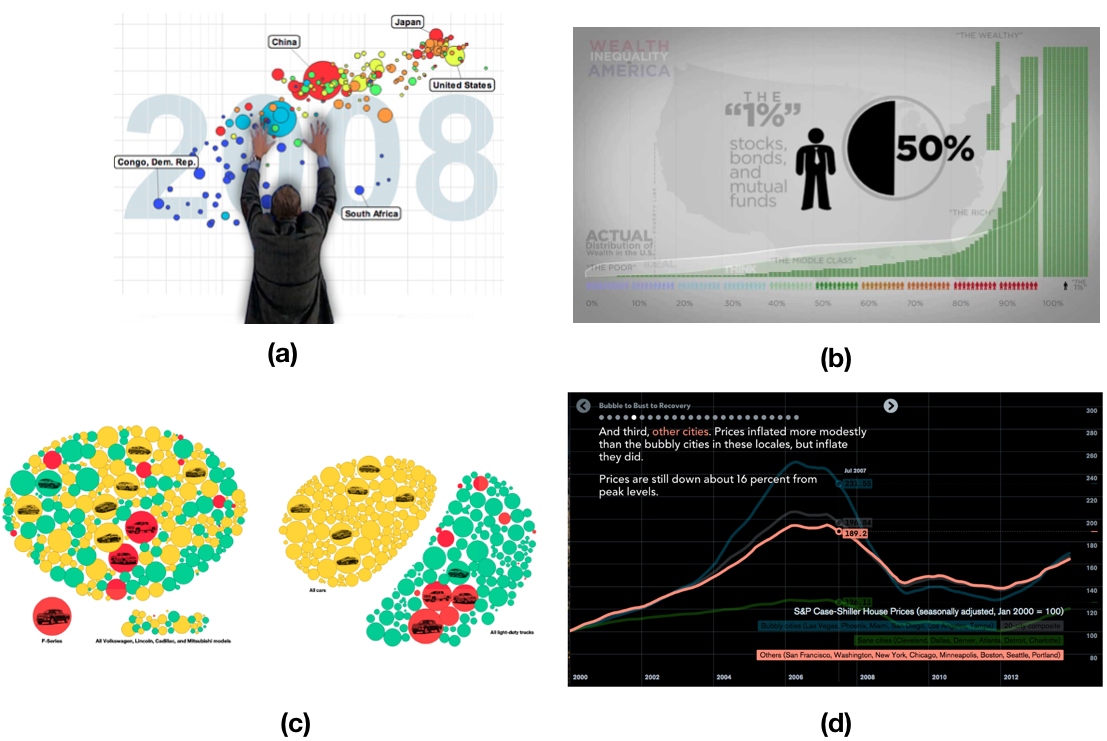
\includegraphics[width=0.95\textwidth]{figure/motivation.png} 
	\caption{Different forms of storytelling. Rosling's talk (a) shows trends in human development \cite{gapminder}. A data video (b) reveals wealth inequality in America \cite{inequality}. Online interactive  visualizations from Bloomberg tell stories such as \textit{Addicted to Trucks} (c) \cite{trunks} and \textit{Bubble to Bust to Recovery} (d) \cite{bust}.} 
	\label{motivation} 
\end{figure}

The current research into data visualization has attached importance to exploratory data analysis. Many visual analytics systems aim to provide novel interfaces and interactions for data exploration, and some also integrate advanced machine learning and data mining algorithms to support powerful analysis ~\cite{May2010}. Comparatively less attention has been paid to the communication function of visualization. However, with the increasing roles of visual data-driven stories and interactive visualization in data analysis, this line of research is attracting interest. The Dagstuhl seminar held in 2016 ~\cite{Carpendale2016} invited both researchers and practitioners to dig into the topic of storytelling using visualization.  Microsoft launched the "data-driven storytelling" project ~\cite{Microsoft}, which aims to understand the story design process and explore methods for easy creation. In spite of several breakthroughs in this field, there is still a plethora of research remaining to be done. For example, although some work ~\cite{Amini2015, Stolper2016, Segel2010} has identified a variety of techniques from existing stories, there is a lack of guidance on how to organize  these techniques given a specific topic. In addition, how to evaluate the effectiveness of not only visual data stories but also visualization authoring tools is yet an open question.


\section{Challenges}
Storytelling is considered as the next step for visualization, specifically for it can present data in an interpretable way ~\cite{Kosara2013}. Thus, we have naturally come to issues of effective visual design in data-driven storytelling. In reference to the design implications informed by good graphics ~\cite{Tversky2002}, visual  design in data-driven narratives should better conform to these two principles as well: one focuses on the content and form of the representation and the other pays attention to the comprehension and perception of the viewers. Therefore, we present three primary challenges resulting from the representation and evaluation of stories, and the limits of authoring tools. 

The first challenge is how to tell stories clearly with engaging visual effects. On the one hand, the mission of a data story is to get a point across and to have the audience understand and trust the content ~\cite{Kosara2013}. Neither describing data and generating insights from an existing dataset nor arranging them in an interpretable way is an easy task.
On the other hand, attractive visual effects contribute to a good narrative. A typical approach is to gain empirical knowledge from a curated collection of data stories. However, the derived design guidance is incomprehensive and constantly evolving. The way to inform an appropriate design space is still under explored.
%Fortunately, storytelling works in a variety of disciplines, leading to theories and practice to produce such effects. It brings a huge opportunity for us to borrow from other fields. However, the way to embed these effects into visual data stories is still under explored.


The second challenge is how to evaluate the effectiveness of such visual data stories. While many interesting stories are widespread and well received in the online media such as Gapminder ~\cite{gapminder} and US wealth inequality ~\cite{inequality}, there is a lack of clearly defined metrics or evaluation methods. Typical measures used in visualization mostly consider time spent on given tasks and their response accuracy through a user study. Nevertheless, these are not pertinent to storytelling, which, instead, requires a crucial evaluation of comprehension, engagement, and memorability of viewers. It also gives rise to problems about comparing the effectiveness of different storytelling techniques. 


Finally, the third challenge is how authoring tools could help support visual narrative designs and lower the barriers to craft data stories. Creating data stories is never a trivial task, relying on a broad set of tools and skills. Authors are expected to use dedicated software or even do the programming themselves when constructing a complete story. Existing tools are limited in many aspects. For example, professional softwares such as Adobe Illustrator or After Effects have steep learning curves and require users' capabilities to design and generate materials. Lightweight tools with a focus on single functions ask for extra tools to complete a story. It is challenging to strike a balance between design flexibility and efficiency of authoring tools. 


\section{Overview}
There are many research issues for transforming data into visually shared stories. However, in this survey, we do not intend to use the term "storytelling" in a broad way that considers all data visualizations as stories. Specifically, this survey mainly focuses on a narrow definition of a visual data story ~\cite{Lee2015}. For example, we exclude exploratory data analysis visualizations which allow users to explore freely and interactively but provide little guidance. In addition, visualizations without enough annotations or written explanations can hardly be considered as well-told stories, since they require viewers to interpret the contents themselves.  Therefore, our analysis is based on asynchronous stories with some form of author-specific narration. Our goal in thie paper is twofold: 1) to review what makes a compelling visual data story based on three primary story components; 2) to investigate ways to author narrative visualization. The rest of this survey is organized as follows.


In Chapter \ref{sec-taxonomy}, we introduce some existing taxonomies for narrative visualization and visual storytelling. After that, we describe our taxonomy derived from the definition of the term "narrative". 


In Chapter \ref{sec-design}, we further illustrate how the visual design in data-driven narratives are developed based on three story components, namely, scenes, sequences, and connection, thus informing the design space. Various techniques are applied in different components to compose compelling and interpretable visual data stories. We then attempt to identify and categorize the design features with collected visualizations.


In Chapter \ref{sec-tool}, we investigate tools to help construct data-driven stories and discuss the evaluation methods used in these visualization authoring tools. 
%Specifically, according to the automatic degree, there exist three kinds of methods to generate visual narrative designs, that is, automatic generation, semi-automated algorithms, and authoring tools.

% In Chapter 4, we categorize core visual narratives based on the surveyed literature from both computer science research and data visualization practice. Particularly, visual narratives mainly facilitate data-driven storytelling in the aspects of trends, ranks, comparisons, relationships, and map presentation.

Finally, we 
%summarize  design implications regarding existing works in Chapter \ref{sec-implication}, and 
conclude some future research directions of visual  design in data-driven narratives in Chapter \ref{sec-conclusion}. 


\newpage
